\chapter{Error Correction Methods}

Since GPS became operational, a range of methodes emerged to improve its positioning accuracy, which were not planned by the inventors of GPS.
These methodes are designed to mitigate the effects of specific errors described in \ref{sec:error_sources}.
Three of the most prominent ones are evaluated in this chapter.
They are rated by how effective they are at improving the accuracy and how well they can be implemented on a sounding rocket.


\section{Dual Frequency Measurements}

A relatively new method of error mitigation for civil GPS users are Dual Frequency Measurements.
This only became possible with the launch of Block IIR-M and IIF satellites.
They transmit a second civilian signal on the L2 frequency called L2C.
The benefit of measuring both the L1 C/A and L2C signal is that the ionospheric delay can be determined.
The ionosphere slows down and radio waves, and thus adds a delay to the measured pseudoranges.
This delay depends on the frequency of the radio wave.
With the difference from pseudorange measurement received on different carrier frequencys, the total ionospheric delay can be calculated.

Dual Frequency Measurements can mitigate the ionospheric error, which is one of the biggest error sources, to a large degree.
This error would otherwise have to be modeled with parameter transmitted by the GPS satellites.
The modeled correction only reduces the error by about 50\%.
Used to implement the dual frequency measurements method are a dual frequency receiver and antenna.
\cite{L1_L2}

\section{Carrier-Phase Measurements}

In standard GPS receivers, the C/A-code is tracked to determine the pseudorange.
The C/A-code is sent out with 1023kbit/s, so each chip is about 300m long.
It is modulated onto the sinusoidal L1-carrier with a frequency of 1575.43MHz.
One period of this carrier is only about 19cm long.
This means the carrier would have a much larger resolution than the C/A-code for tracking.
Receiver who use this principle measure the carrier-phase.
The problem with this is the periodical nature of the carrier.
The phase can be measured very precisely, but it can not be directly measured how many whole cycles are between the user and the satellite.
This ambiguity has to be resolved in other ways before the carrier-phase measurement can be used, which can take some time.
After the ambiguity is resolved, the carrier has to be continuously tracked to count the whole cycles.
With the higher resolution, the tracking error introduced by receiver noise can be reduced.

\begin{figure}[ht]
 \centering
 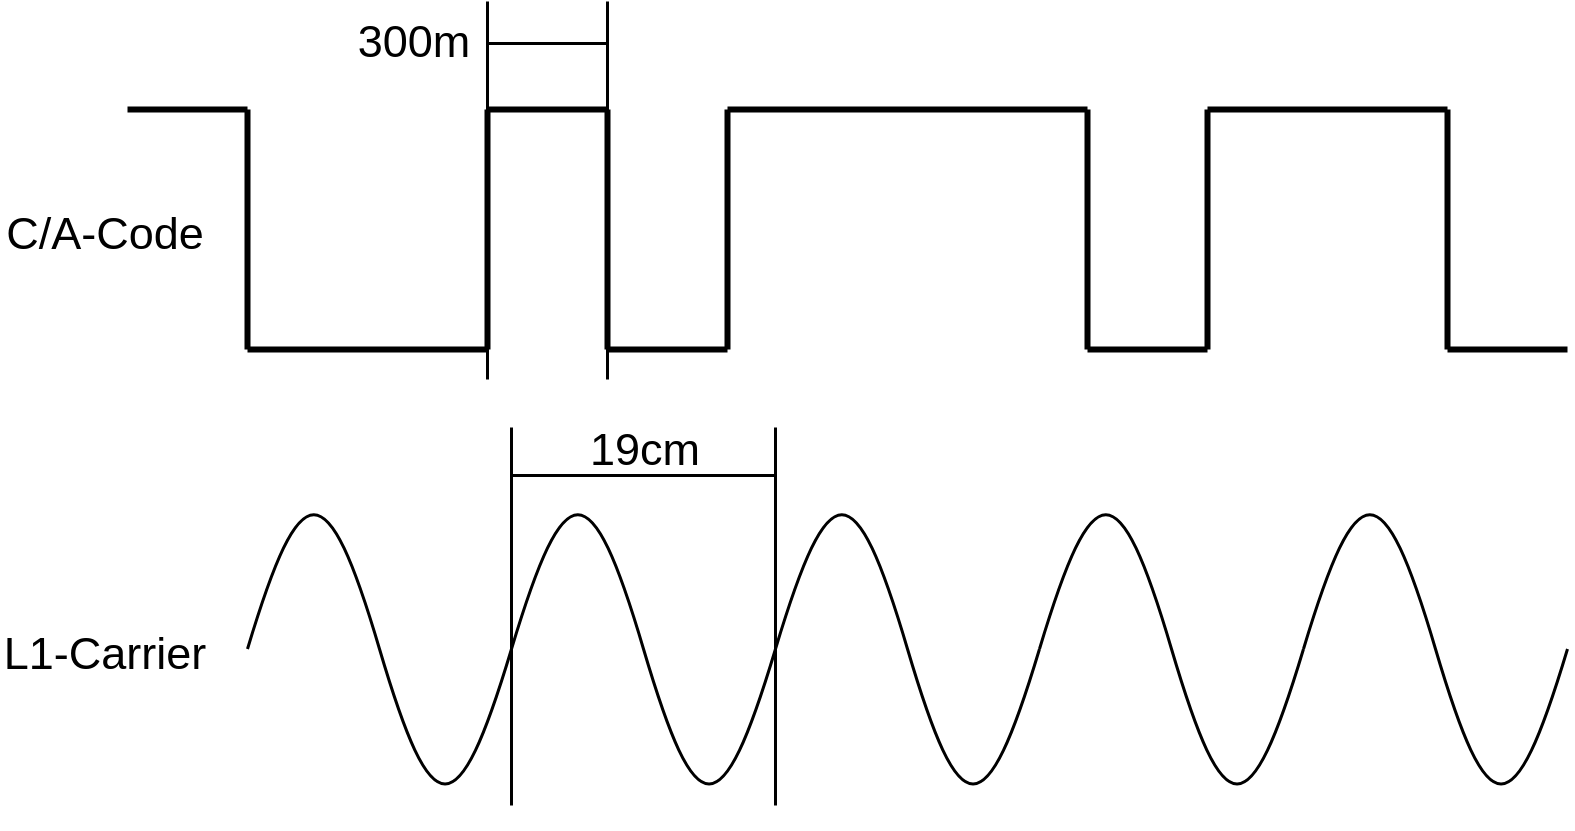
\includegraphics[height=5cm]{images/Carrier-Phase_Measurement.png}
 \caption{Difference in resolution between C/A-code and L1-carrier}
 \label{fig:carrier_phase}
\end{figure}

Carrier-phase measurements also improve multipath.
The advantage is that reflected signals with a delay of more than a quarter cyrcle do not impact the measurement.
In the case of the L1-carrier, this is only about 5cm.
A typical multipath error for C/A-code measurements is 1-5m.

\section{Differential GPS}

\section{Summary}